\documentclass[assignment01_Solutions]{subfiles}

\IfSubStr{\jobname}{\detokenize{Solutions}}{\toggletrue{solutions}}{\togglefalse{solutions}}

\fancypagestyle{firstpage}

{\rhead{Assignment 1 \linebreak \textit{Version: \today}}}

\title{Assignment 1: Bayes' Rule}
\author{Machine Learning}
\date{Fall 2019}

\begin{document}

\maketitle
\thispagestyle{firstpage}


\begin{learningobjectives}
\bi
\item Learn about some big deas in Bayesian Machine Learning.
\item Define the concept of a probability.
\item Learn Bayes' rule and other rules for manipulating probabilities.
\item Use a computational framework to apply Bayes' rule to simple problems.
\ei
\end{learningobjectives}

\section{Motivation}
The theme of uncertainty has cropped up a number of times so far this semester.  For instance, we learned about the logistic regression model, which computes the probability that the output for a given input is 1.  In this way, the model explicitly represents the uncertainty of its predictions and uses the concept of probability to express this uncertainty.  We’ve also seen examples of models that don’t fit the data perfectly (well that's pretty much every model!).  For example, the plot in Figure~\ref{fig:lineofbestfit} shows a line of best fit that doesn't go through all of the data.  The fit might be imperfect because we don't have the right model (a form of uncertainty) or because the thing we are trying to predict is inherently random in some way (another form of uncertainty).
\begin{marginfigure}
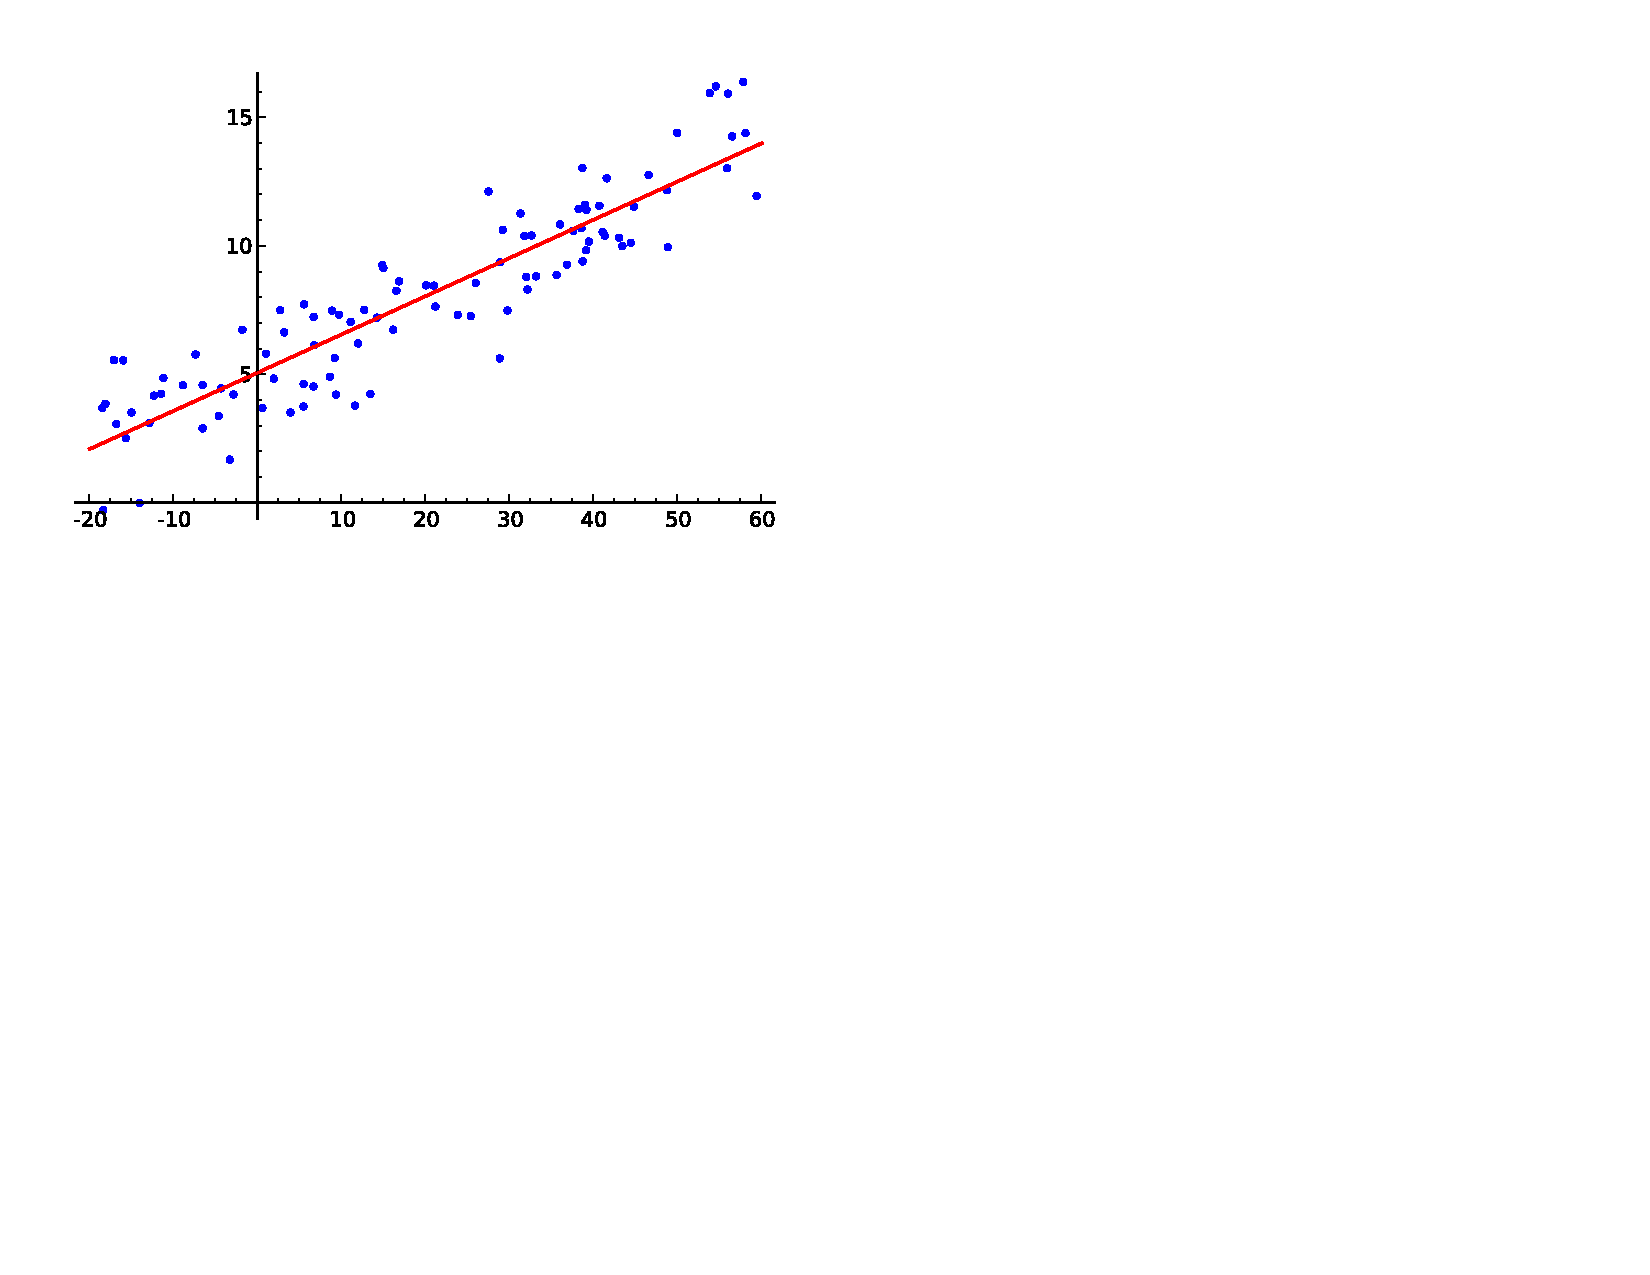
\includegraphics[width=\linewidth]{figures/line_of_best_fit.pdf}
\caption{A dataset with one independent variable and one dependent variable.  Also shown is the line of best fit.\label{fig:lineofbestfit}}
\end{marginfigure}


It turns out that the notion of probability provides us with a powerful method to formalize the concept of uncertainty and allows us to reason about many types of uncertainty in a unified way.  Formalizing uncertainty using probability theory will enable us to do a bunch of really cool things with respect to machine learning, including

\bi
\item make explicit our assumptions about where data comes, the uncertainties present within it, and the impact of uncertainty on predictions based on that data.
\item allow us to quantify our confidence in our model.  For example, instead of returning the one best fitting model (as we did in the first module), we assign a probability to each possible model, and models that fit the data better will get a higher probability.
\item give us a way to incorporate expert knowledge into our machine learning models.  This expert knowledge can allow for us to learn more interpretable and accurate models.
\item give us powerful tools to reason about fairness and bias in machine learning models.
\ei

\section{Six Big Ideas in (Probabilistic) Machine Learning}
Back by popular demand\sidenote{there was actually no specific demand for this, but we couldn't resist :).}... here are Six (more) Big ideas in ML!  Here we're going to highlight ideas in ML that have specific connections to Bayesian machine learning.

\begin{notice}
Our intent is to provide a larger framework for you to interpret the content you are learning.  You should not expect to understand all of these ideas in any sort of detail.  Please take these as a ``wow isn't this cool / interesting,'' and avoid getting too lost in the weeds.
\end{notice}


\begin{exercise}[\faShareAlt~(60 minutes)]
Read the six big ideas in ML below.  You will choose one of them and write a short response to it.  Your response could incorporate something surprising you read, a thought-provoking question, your personal experience, an additional resource that builds upon or shifts the discussion.  We hope that this reflection will help scaffold class discussions and get you thinking about your interests in the big space that is ML.  Also, you have license from us to customize the structure of your response as you see fit.  Aim for a response of about one longish paragraph.

\begin{boxedsolution}
There's no one right answer here!
\end{boxedsolution}
\end{exercise}


\subsection*{Idea 1: Bayesian Methods Can Illuminate Hidden Structures}

One task in which Bayesian machine learning shines is in determining the hidden structures that underlie data.  One very cool example of this is in the field of \href{https://en.wikipedia.org/wiki/Bioinformatics}{bioinformatics}.  A key idea in evolutionary biology is the notion of a \href{https://en.wikipedia.org/wiki/Phylogenetic_tree}{phylogenetic tree}.  A phylogenetic tree captures the relationships between various entities (e.g., individual members of a species, different species, genes, etc.) in a hierarchy (or tree).  For instance, the figure below shows a phylogenetic tree of the vertebrates.

\begin{center}
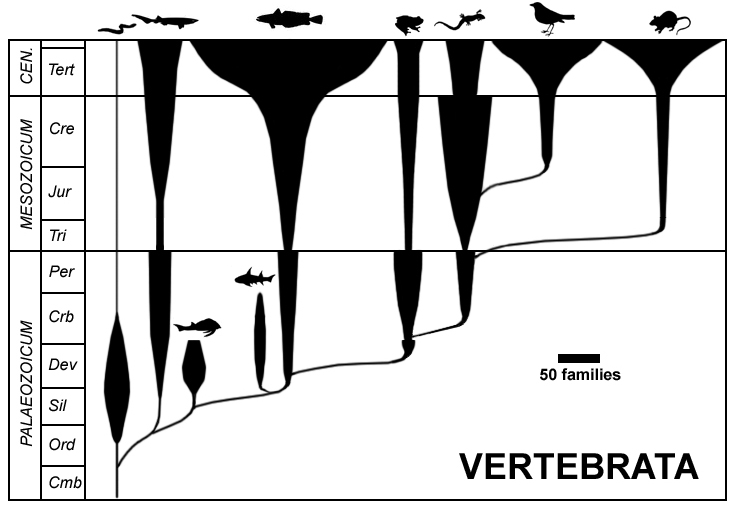
\includegraphics[width=0.8\linewidth]{figures/vertebrates}
\end{center}

This tree not only shows which families of vertebrates evolved from other families, but also provides an approximate timeline when these branching occurred.  Such a phylogenetic tree would be built using a combination of fossil records along with analysis of modern day versions of these species.  It turns out that Bayesian machine learning is a key tool that is used to automatically infer phylogenetic trees from a wide variety of data sources.  One example is combining \href{https://en.wikipedia.org/wiki/Mitochondrial_DNA}{mitochondrial DNA} collected from people all around the world with machine learning analysis to reconstruct the most likely phylogenetic tree that underlies these DNA samples.  The result is an ancestral tree that helps reconstruct the ancient history of humans and provides a snapshot of how they came to inhabit planet Earth.  Reconstructions of this type have given support to the ``out of Africa'' theory, which states that all people alive today can trace their lineage back to a group of people in sub-Saharan African about 150,000 - 200,000 years ago.

Bayesian approaches to inferring phylogenetic trees have been used in a vast number of places.  The abstract of \href{https://www.ncbi.nlm.nih.gov/pmc/articles/PMC5624502/}{A biologist’s guide to Bayesian phylogenetic analysis} describes it in the following way.
\begin{quote}
Bayesian phylogenetic methods were introduced in the 1990s and have since revolutionised the way we analyse genomic sequence data. Examples of such analyses include phylogeographic analysis of virus spread in humans, inference of phylogeographic history and migration between species, analysis of species diversification rates, divergence time estimation, and inference of phylogenetic relationships among species or populations.
\end{quote}

The concept of a phylogenetic tree has even been used used in linguistics as a mechanism to study \href{https://journals.plos.org/plosone/article?id=10.1371/journal.pone.0180908}{the evolution of languages over time}.

\paragraph{(If You're Interested): More examples of finding hidden structures in data}

\href{https://homes.cs.washington.edu/~rao/ScienceIndus.pdf}{Entropic Evidence for Linguistic Structure in the Indus Script}

\subsection*{Idea 2: Bayesian Methods Allow Us to Write Probabilistic Programs}

The key idea of Bayesian machine learning is that we can take causal models of how hidden structures give rise to observable data and invert them to allow us to use data to reason about the hidden structures that caused that data.  One of the coolest ways in which this fundamental idea is being utilized is in the field of \href{https://en.wikipedia.org/wiki/Probabilistic_programming}{probabilistic programming}.  In a probabilistic program, the programmer writes code to implement the causal model (the one that goes from hidden structures to data).  In contrast to a typical program where we might take a particular input and produce a single output, a probabilistic program specifies a random process by which data is generated.  Uncertainty is represented explicitly at each step in the program.  Once the programmer has specified the causal model for how data is generated, the probabilistic programming framework can automatically infer the hidden structure given a sample of data!

For instance, one of the examples for the popular probabilistic programming library \href{https://docs.pymc.io/}{pymc3} shows how a model of CO2 concentration in the atmosphere could be created using a probabilistic program (see \href{https://docs.pymc.io/notebooks/GP-MaunaLoa.html}{Mauna Loa CO2 example}).  The punchline graph from that notebook is reproduced below.  In this case the programmer had to specify the process by which underlying phenomena (e.g., increases in CO2 levels globally, seasonal factors) give rise to observable data (CO2 measurements at the top of Mauna Loa).  This probabilistic program was then given atmospheric data up to 2004 and pymc3 automatically generated predictions for the CO2 data from 2004 onwards.  In addition to the curve shown below, the model was able to decompose the curve into various components (including long range and seasonal effects).  You may notice the fit is not perfect.  There is \href{https://docs.pymc.io/notebooks/GP-MaunaLoa2.html}{a more advanced example} that achieves a better fit and leverages ice core data.

\begin{center}
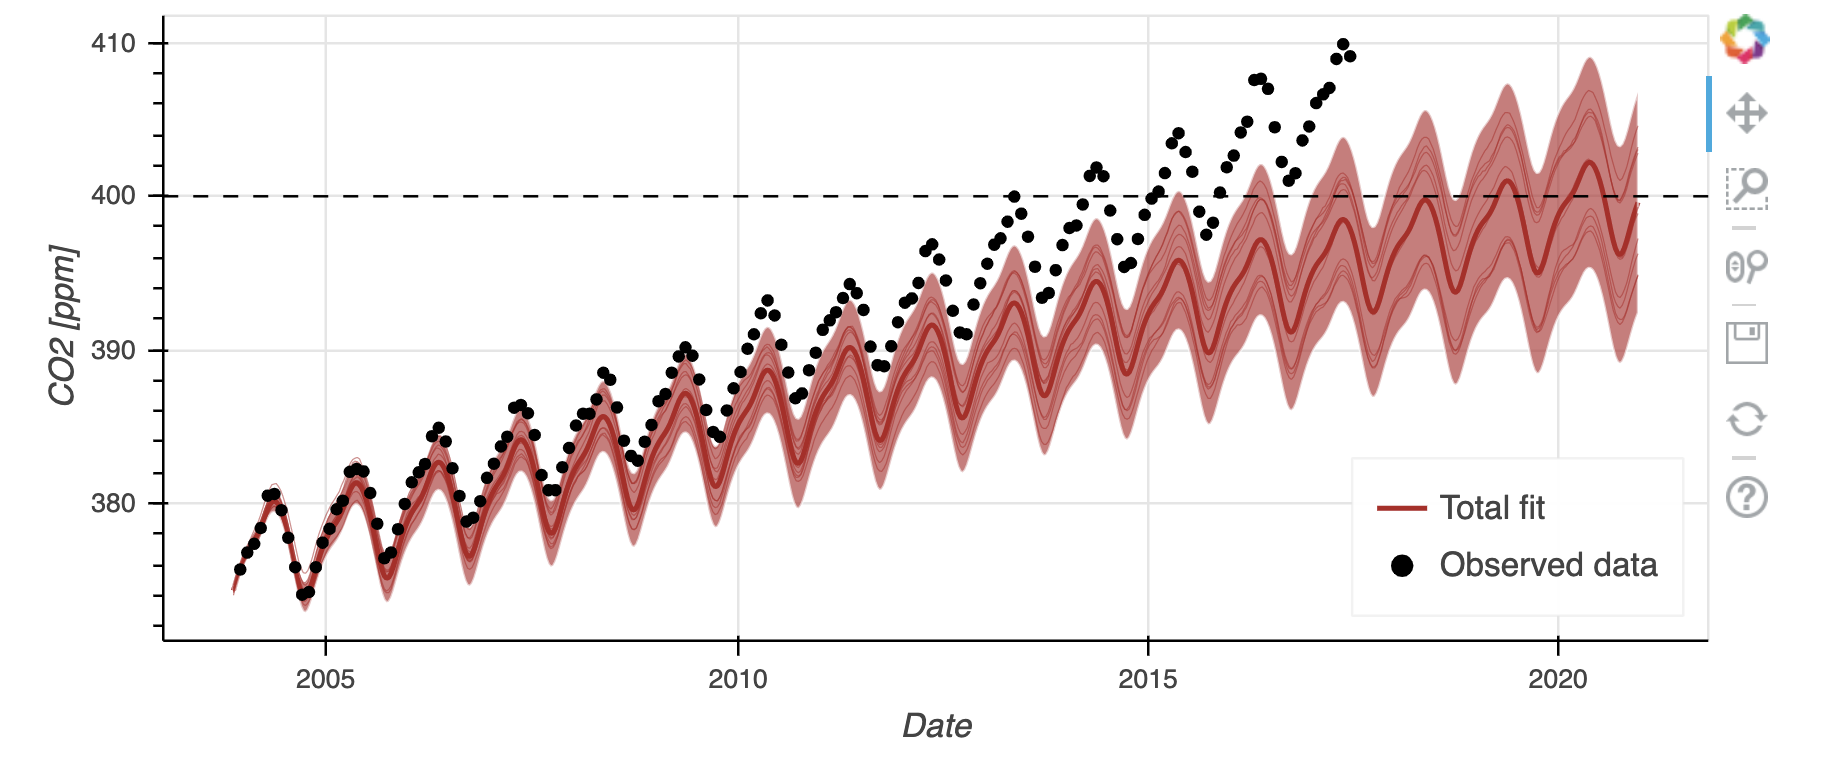
\includegraphics[width=0.8\linewidth]{figures/maunaloa}
\end{center}

\paragraph{(If You're Interested): Here are some more examples of probabilistic programming}
Is computer vision really just inverse computer graphics?  If you use probabilistic programming you can simply specify the forward model of how objects in a scene give rise, probabilistically, to an image. Probabilistic programming can then take an image and infer the underlying structure that gave rise to a test image.  Examples of this include fitting  \href{http://mrkulk.github.io/www_cvpr15/}{3D models to human faces} (follow the link to some cool videos) and \href{https://science.sciencemag.org/content/sci/360/6394/1204.full.pdf}{predicting how a geometric scene would look from an arbitrary vantage point from a single training image}.


\subsection*{Idea 3: Bayesian Methods Can Help Us Understand Learning and Perception in Humans and Robots}

One common challenge that humans and robots (and other animals for that matter) face is the need to interpret ambiguous information in the world around them.  For instance, the photons of light that hit our retinas create a 2D map of a 3D world.  Despite the fact that there are many possible 3D worlds that could have created the same pattern of light on our retinas, our brain, for the most part, has no trouble figuring out the correct 3D structure of the world\sidenote{optical illusions are a good example of when this does not hold (i.e., our brain is tricked into inferring the wrong 3D structure).}.

One approach that scientists have taken to understand how humans accurately extract structure in the face of ambiguous information is by applying what is known as the \href{https://www.cse.huji.ac.il/~yweiss/intro/node2.html}{computational approach}.  In the computational approach, one formalizes the goal of the agent as well as the constraints facing it.  For example, perhaps a person is trying to accurately understand the 3D structure of their environment but is constrained to only have access to a 2D projection of that environment (i.e., the 2D projection is what is captured on our retina).  Once we have formalized the problem facing the agent, we can then use computational tools to compute the optimal solution to the problem and compare this solution to what people actually do.  Through this comparison we may learn more about the nature of human cognition and the reasons why humans think and act the way they do.  In David Marr's classic work ``Vision,'' he states the core idea in the following way.

\begin{quote}
Trying to understand perception by studying only neurons is like trying to understand bird flight by studying only feathers: It just cannot be done. In order to understand bird flight, we have to understand aerodynamics; only then do the structure of feathers and the different shapes of birds' wings make sense. [Marr, 1982] p. 27
 \end{quote}

The science of ``aerodynamics'' is being invoked in the quote to reference a fundamental theory that governs all systems that might try to fly.  When it comes to cognition, the idea of Bayesian inference, which will form the basis of Bayesian machine learning, has increasingly emerged as the ``aerodynamics'' of thought and reasoning.  Scientists and engineers have used Bayesian approaches to understand a vast array of human cognition and behavior.

\bi
\item \href{https://www.sciencedirect.com/science/article/pii/S0022249615000061}{Sensory perception}
\item \href{https://www.nature.com/articles/nn963}{Motor control}
\item \href{http://web.mit.edu/cocosci/Papers/Science-2011-Teglas-1054-9.pdf}{Babies can use Bayesian inference to understand physics... sort of}
\item \href{https://www.ncbi.nlm.nih.gov/pubmed/24730598}{The tendency of people to with divergent beliefs to become more polarized when presented with the same evidence (think current politics)}
\item \href{https://www.sciencedirect.com/science/article/pii/S0022249608001090}{How people behave in a simulated gambling environment}
\item \href{https://arxiv.org/abs/1806.03916}{How people ascribe trust to others}
\item \href{https://www.sciencedirect.com/science/article/pii/S1364661306001318}{How people acquire language}
\ei


\subsection*{Idea 4: Bayesian Methods Give Us a Language for Reasoning about Algorithmic Fairness}

We've talked about bias in machine learning models (e.g., when we discussed Gender Shades).  The examples given in the \href{http://gendershades.org/overview.html}{Gender Shades} paper were pretty cut-and-dry --- the commercial gender classification models work very poorly on women and people of color (and especially the intersection of the two).  In other situations it is not so straightforward to reason about bias. For instance, in the well-known ProPublica piece \href{https://www.propublica.org/article/machine-bias-risk-assessments-in-criminal-sentencing}{Machine Bias} the authors describe how a tool for predicting criminal recidivism (whether a criminal would reoffend) was biased against African Americans.  This piece was important in the field of FAT-ML in that it sparked work on articulating various definitions of algorithmic fairness (these notions were sometimes, inherently, inconsistent).  Most of these models of fairness are articulated using the language of probability.  Further, some of the same formalisms that have been used to develop probabilistic machine learning approaches can be used to understand and reason about bias in an algorithm.

We'll be studying various notions of algorithmic fairness, but if you're interested, an in-depth overview of this is provided in \href{https://arxiv.org/pdf/1906.11333.pdf}{Fairness criteria through the lens of directed acyclic graphical models}.  It's also worth mentioning that many of these notions of fairness have also been challenged on the grounds that they are overly abstract and gloss over important context in determining whether something is biased or not.


\subsection*{Idea 5: Bayesian Methods Allow for Learning More Interpretable and Flexible Models}

Since Bayesian models typically start from a causal model of how observable data are generated, when this process is inverted, you are left with an understanding of the most probable causes of the data you observed.  Oftentimes this output is easier to interpret than what might be generated by, say, a neural network, which has no explicit causal model of data generation.  As a motivating example, take for example the usage of computers to help doctors diagnose patients (this is sometimes called a \href{https://en.wikipedia.org/wiki/Clinical_decision_support_system}{Clinical Decision Support System}).  Here are two ways in which we might tackle this problem using neural networks versus Bayesian machine learning.

\bi
\item Neural networks: we would get a dataset of tons of patients, their symptoms, and their diagnoses.  We would train a neural network model to map from symptoms to diagnoses.
\item We would have an explicit model of how underlying factors (e.g., diseases, age, environmental conditions) give rise to symptoms.  We would fit some of the parameters of that model using clinical data or through prior knowledge (e.g., the intuition of doctors).  When we wanted to diagnose a patient, we would use Bayesian inference to predict the likely underlying disease that contributed to the patient's symptoms.
\ei
 
One potential advantage of the Bayesian approach is that its decisions might be more understandable / familiar to a doctor (since its process is not that different from how a doctor might diagnose patients themselves).  Further, if some aspect of the environment changed (e.g., the sensitivity of a test for a disease increased or the prevalence of a disease decreased), the predictions would naturally adjust.  It is less easy to see how to incorporate these sorts of changes into the neural network approach.
 
 \begin{marginfigure}
 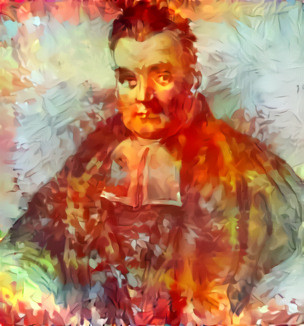
\includegraphics[width=\linewidth]{figures/bayesdeepdream}
 \caption{Bayes (pictured) meets neural networks.  Generated using \href{https://deepdreamgenerator.com}{deepdreamgenerator.com}}
 \end{marginfigure}
 This is not to bash neural networks!  There is even a burgeoning field designed to \href{https://alexgkendall.com/computer_vision/bayesian_deep_learning_for_safe_ai/}{bring some of the advantages of Bayesian approaches} to the field of deep learning.  A figure from this work is shown below.  The network in question is able to represent not only its prediction regarding the likely depth map (center) given a stereo image (left), but also the uncertainty that the model has for various parts of the image (right).
 
 \begin{center}
  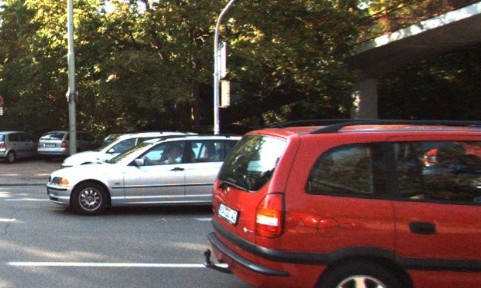
\includegraphics[width=0.3\linewidth]{figures/left_stereo}
    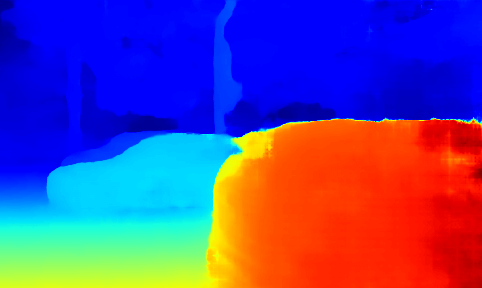
\includegraphics[width=0.3\linewidth]{figures/disparity}
 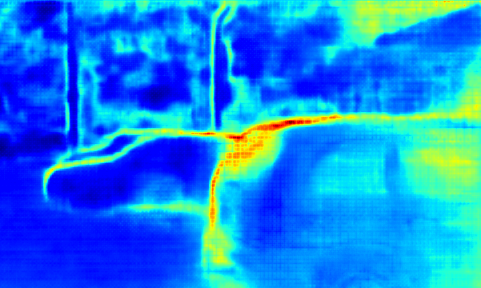
\includegraphics[width=0.3\linewidth]{figures/depthuncertainty}
 \end{center}

\subsection*{Idea 6: Bayesian Methods Pose Difficult Computational Challenges}
While we've painted a fairly rosy picture of Bayesian methods, they are certainly not without their challenges.  One of the biggest challenges is computational (see here for \href{https://link.springer.com/article/10.1007/s11222-015-9574-5}{a summary of current computational challenges in Bayesian learning}).  The key reason that Bayesian methods can be computationally expensive is that they involve solving the following sorts of problems.
\bi
\item Bayesian methods involve inverting causal models of the world.  This inversion process may not be well-posed and could result in very inefficient computations.
\item Bayesian methods involve representing uncertainty over large model spaces.  Just representing this model space, let alone using it for making predictions can be hard.
\ei
Therefore, while Bayesian methods are very attractive (and will pose no significant computational problems in some important special cases, which we will learn about in this module), efficiently using Bayesian methods is an active area of research.

\section{Probability}

Hopefully the previous section left you feeling excited to learn more about the theory that underlies these big ideas.  Next, we'll take our first steps towards learning this theory.

\subsection{Intuition}
Most of us are used to thinking that events can be probabilistic, that is we can attach some probability to whether or not they occur.  Take for example flipping a coin.  We could think of the event that the coin comes up heads as having probability 0.5.  That is, there is an even chance that it happens versus doesn’t happen.  Further, we can say that an event is \emph{observable} if we are able to directly observe whether it occurred.  For instance, whether a coin comes up heads is an observable event since you can ultimately observe the outcome of the flip.  In contrast, some events would be considered unobservable if they are unable to be directly ascertained by human senses.  A classic example of this would be whether a scientific theory is true or not.  It is impossible to directly observe whether the theory is true, but you might be able to observe events that are consistent or inconsistent with the theory.

\vspace{1em}
\begin{exercise}[(10 minutes)]
Come up with 3ish examples of observable events that are probabilistic in nature.  For each event, provide the probability that it occurs or explain what factors would determine the probability.  Some potential ideas to get you going: sporting events, elections, weather, etc.

\begin{boxedsolution}
Here are some possible ideas.
\bi
\item The event \emph{The Nationals win the 2019 MLB World Series} is an observable event (we will ultimately find out whether or not this happens).  The probability of this event will depend on the quality of their opponent (currently this is either the Yankees or the Astros, both of whom would be favored in the series) and other factors (such as home field advantage).
\item The event the movie Joker wins the Academy Award for Best Pictures is an observable event.  The probability that it occurs will depend on the amount of money spent promoting it to academy members, the quality of other movies that are released, etc.
\ei
\end{boxedsolution}

\end{exercise}

\subsection{Formal Definition}

Next, we'll define more formally\sidenote{this is not the full definition of a \href{https://en.wikipedia.org/wiki/Probability_space}{probability space} used in modern mathematics.  For the purposes of most people that \emph{use} probability theory on actual problems, the full definition is needlessly complex.  For instance, as a grad student I (Paul) never saw the full definition in any of my ML courses.  Use the following link if you want a more \href{https://m.tau.ac.il/~tsirel/dump/Static/knowino.org/wiki/Probability_space.html}{in-depth discussion of the parts of the formal definition that are tricky} (our expectation is that you won't want this discussion!).} what we mean by a probability.  Having this formal definition will give us the ability to determine useful rules for manipulating and reasoning about probabilities.  To define the concept of a probability, we'll need to specify two ingredients.
\subsection{Events}

An \emph{event} is something that may or may not occur in response to some random process.  For instance, we could define the event that a coin comes up heads when it is flipped.  We often use capital letters to indicate events.  Since we've been using capital letters to also represent matrices, in our materials we'll use a cool mathy-looking calligraphic font to represent events.  For instance, we might use the symbol $\mathcal{H}$ to refer to the event that a coin flip comes up heads. It's important to emphasize that a single random process can have many associated events.   For instance, for the coin flip example we might also define $\mathcal{T}$ to be the event that the coin comes up tails (or $\mathcal{U}$ to indicate that event that the coin rotated at least 10 times in the air when we flipped it).

Further, events don't necessarily have to be mutually exclusive.  For instance, we might define the event $\mathcal{R}_h$ to indicate the event that the Republican party controls the majority in the House of Representatives following the 2020 election and $\mathcal{D}_s$ to indicate the event that the Democratic party controls the majority in the Senate following the 2020 election.  Both (or none) of these events could occur.

\subsection{Probability Measure Function}
The probability measure function assigns a probability to the occurrence of any particular event.  We can think of this probability measure function as taking as input an event and outputting a probability.  For instance, $p(\mathcal{E})$ provides the probability that event $\mathcal{E}$ occurs according to probability measure $p$.  All probability measure functions must satisfy the following properties.

\bi
\item $0 \leq p(\mathcal{E}) \leq 1$: the probability of an event ranges from 0 (an impossible event) to 1 (an event that will always occur).
\item Given a set of $n$ events $\mathcal{E}_1, \mathcal{E}_2, \ldots, \mathcal{E}_n$ that are disjoint (i.e., no two can occur simultaneously)
\begin{align}
p(\mathcal{E}_1~\mbox{or}~\mathcal{E}_2~\mbox{or}~\ldots~\mbox{or}~\mathcal{E}_n) = \sum_{i=1}^n p(\mathcal{E}_i) \label{eq:probunion} \enspace .
\end{align}


The equation above specifies what is sometimes called the union rule of probability.  It states that the probability of one of these disjoint events occurring must be equal to the sum of the probability of each of the events occurring.  You will also sometimes see Equation~\ref{eq:probunion} written as

\begin{align}
p(\mathcal{E}_1 \cup \mathcal{E}_2 \cup \ldots \cup \mathcal{E}_n) = \sum_{i=1}^n p(\mathcal{E}_i) \enspace .
\end{align}

If you're not familiar with the symbol $\cup$ it is the symbol for a union of two sets.  The reason you'll sometimes see this notation is that in the full definition of a probability space an event is defined as a set (as stated in the margin note earlier in this section, you need not worry about the most rigorous definition in this course).

\item Given a set of (not necessarily disjoint) events $\mathcal{E}_1, \mathcal{E}_2, \ldots, \mathcal{E}_n$ where at least one of these $n$ events must occur
\begin{align}
p(\mathcal{E}_1~\mbox{or}~\mathcal{E}_2~\mbox{or}~\ldots~\mbox{or}~\mathcal{E}_n) = 1 \enspace .
\end{align}
\ei

This rule just states that if we have an exhaustive set of events (that cover all possible cases), at least one of them \emph{must} occur.

\subsection{Complement Rule for Probability}

Given the definition of probability detailed above, it follows that if the probability of an event happening is $p(\mathcal{E})$ then the probability of the event \emph{NOT} happening is $1-p(\mathcal{E})$.   The following are common ways of to express this relationship (we'll use Equation~\ref{eq:complement} in this class).  These all say the same thing (the only difference is notation).

\begin{align}
p(\neg \mathcal{E}) &= 1 - p(\mathcal{E}) \label{eq:complement} \\
p(\mbox{not}~\mathcal{E}) &= 1 - p(\mathcal{E}) \nonumber \\
p(\overline{\mathcal{E}}) &= 1 - p(\mathcal{E}) \nonumber \\
p(\mathcal{E}') &= 1 - p(\mathcal{E}) \nonumber \\
p(\mathcal{E}^c) &= 1 - p(\mathcal{E}) \nonumber
\end{align}

We point out these alternate notations not to confuse you (we'd never do that!) but to help you interpret various external resources you might find on these topics.

\vspace{1em}
\begin{exercise}[(10 minutes)]
Here are some diagnostic questions to make sure that you got the basic ideas. 
\bes
\item Suppose $\mathcal{E}_1, \mathcal{E}_2, \mathcal{E}_3$ are disjoint events.  Further, suppose that one of these events must occur.  Which of the following functions are valid probability measure functions?

\begin{align}
p_1(\mathcal{E}_1)=\frac{1}{10} , p_1(\mathcal{E}_2)=\frac{1}{5}, p_1(\mathcal{E}_3)=\frac{7}{10} \nonumber
\end{align}


\begin{align}
p_2(\mathcal{E}_1)=\frac{11}{10} , p_2(\mathcal{E}_2)=\frac{-1}{10}, p_2(\mathcal{E}_3)= 0 \nonumber
\end{align}



\begin{align}
p_3(\mathcal{E}_1)=\frac{1}{10} , p_3(\mathcal{E}_2)=\frac{1}{5}, p_3(\mathcal{E}_3)=\frac{1}{2} \nonumber
\end{align}



\begin{align}
p_4(\mathcal{E}_1)=1 , p_4(\mathcal{E}_2)=0, p_4(\mathcal{E}_3)=0 \nonumber
\end{align}

\begin{boxedsolution}
$p_1$ is a valid probability measure function since the probabilities add up to 1 and all are non-negative.  $p_2$ is not a valid probability measure function since two of the probabilities are outside of the appropriate range $[0,1]$.  $p_3$ is not a valid probability measure function since the probabilities of the three events add up to less than 1. $p_4$ is a valid probability measure function since the probabilities add to 1 and are in the appropriate range.
\end{boxedsolution}

\item The Birthday Problem is a well-known probability problem often used in discrete math courses.  According to \href{https://en.wikipedia.org/wiki/Birthday_problem}{the Wikipedia article on the Birthday Problem}, the probability that at least two students among the 70 students in machine learning this semester share the same birthday is $0.999$.  What is the probability that no two students share the same birthday?

\begin{boxedsolution}
Notice that the event \emph{no two students share a birthday} only happens when the event \emph{at least two students share a birthday} does not happen.  Therefore, these events are complements.

\begin{align}
p(\mbox{no two students share a birthday}) &= 1 - p( \neg \mbox{no two students share a birthday})  \nonumber\\
&= 1 - p(\mbox{at least two students share a birthday}) \nonumber \\
&= 1 - 0.999  \nonumber\\
&= 0.001  \nonumber
\end{align}
\end{boxedsolution}

\ees
\end{exercise}

\section{Bayes' Rule}

\begin{externalresources}[(60 minutes)]
\begin{learningobjectives}
Note that these learning objectives have been written to be very specific (based on feedback from the course survey).  When you first read them, you probably won't know what they mean in detail.  As you go through the readings, hopefully the more precise statement of these learning objectives will be useful for assessing your understanding of the provided resources.

\bi
\item When Bayes' rule is useful (i.e., when $p(A|B)$ is easier to work with than $p(B|A)$).
\item The idea of a conjoint probability $p(\mathcal{A}, \mathcal{B})$ (note: alternate notations include $p(\mathcal{A}~\mbox{and}~\mathcal{B})$ and $p(\mathcal{A} \cap \mathcal{B})$).
\item The definition of a conditional probability $p(\mathcal{A} | \mathcal{B}) = \frac{p(\mathcal{A},\mathcal{B})}{p(\mathcal{B})}$.
\item The equation for the product rule $p(\mathcal{A}, \mathcal{B}) = p(\mathcal{B}) p(\mathcal{A} | \mathcal{B}) =  p(\mathcal{A}) p(\mathcal{B} | \mathcal{A})$ (Allen calls this the probability of a conjunction).
\item The equation for Bayes' rule $p(\mathcal{A} | \mathcal{B}) = \frac{p(\mathcal{B} | \mathcal{A}) p(\mathcal{A})}{p(\mathcal{B})}$.
\ei
\end{learningobjectives}

Allen Downey (ever heard of him?) wrote an excellent book called Think Bayes that introduces Bayesian analysis.  The \href{http://www.greenteapress.com/thinkbayes/html/thinkbayes002.html}{first chapter} (which you should read) starts with a less formal definition of probability than the one we gave earlier.  The chapter then gives intuitions around conjoint probability (the probability that multiple events occur simultaneously), conditional probability (the probability that some event occurs conditioned on another event having occurred), and finally to Bayes' rule (a surprisingly easy theorem to derive that allows you to write one conditional probability distribution in terms of another).  The Monty Hall problem in section 1.7 is probably okay to skim (see Allen's note at the end of that section for why this is the case).

Allen's treatment of the material is, of course, not the only one out there (we like it for its focus on building intuition and focusing on the key ideas).  Here are some other resources you might consider checking out (they are optional).
\bi
\item \href{https://www.khanacademy.org/partner-content/wi-phi/wiphi-critical-thinking/wiphi-fundamentals/v/bayes-theorem}{Khan Academy Video on Bayes' Theorem} shows some simple applications of Bayes' rule and explains why it is a convenient way to reason about the probability of hypothesis given data).
\item \href{https://www.youtube.com/watch?v=R13BD8qKeTg}{Veritasium Episode on Bayes' Theorem} has a bit more history and philosophy of Bayes' Theorem along with some nice visualizations.  It also includes the presenter walking on a very scenic mountain (for some reason), so there's that if nothing else.
\item Julia Galef's video \href{https://www.youtube.com/watch?v=BrK7X_XlGB8}{A Visual Guide to Bayesian Thinking}
\item I (Paul) ran across \href{https://youtube.com/watch?v=nvqXXlz-rx0}{this example of applying Bayes' rule to a real world problem}.  It was created by a grad school friend of mine and is hilarious (lots of Cat Memes).  I did notice that there is a mistake in the math at the 8:12 mark in the video (he states that $p(\mbox{alarm} | \mbox{no theft}) = 1 - p(\mbox{alarm} | \mbox{theft})$, which is not necessarily the case).  It's still a good video though.
\ei

\end{externalresources}

\begin{exercise}[(20 minutes)]
\begin{notice}
If you are having trouble dealing with the denominator that you get when you apply Bayes' rule, you may want to skip ahead to the section on the \emph{Marginalization Rule for Probabilities} and then return to these problems.
\end{notice}
\bes
\item You are given three coins.  Two are of type 1, we'll call this type $\mathcal{C}_1$, and one is of type 2, we'll call this type $\mathcal{C}_2$. If you flip a coin of type 1, the coin will come up heads with probability $\frac{4}{5}$ (i.e., $p(\mathcal{H} | \mathcal{C}_1) = \frac{4}{5}$). If you flip a coin of type 2, the coin will come up heads with probability $\frac{1}{2}$ (i.e., $p(\mathcal{H} | \mathcal{C}_2) = \frac{1}{2}$).  Suppose you choose one of the three coins (there is no way for you to tell them apart), flip it once, and it comes up heads.  What is the probability that you flipped a coin of type 2 (i.e., what is $p(\mathcal{C}_2 | \mathcal{H})$)?  After you compute your answer, compare it with the probability that a randomly selected coin was of type 2 (before you flipped it and observed heads).  Does the relationship between this prior probability and the posterior probability make sense?

\begin{boxedsolution}
\begin{align}
p(\mathcal{C}_2 | \mathcal{H}) &= \frac{p(\mathcal{H} | \mathcal{C}_2) p(\mathcal{C}_2)}{p(\mathcal{H})} & \mbox{Bayes' Rule} \nonumber \\
&=  \frac{p(\mathcal{H} | \mathcal{C}_2) p(\mathcal{C}_2)}{p(\mathcal{C}_1) p(\mathcal{H}|\mathcal{C}_1) + p(\mathcal{C}_2) p(\mathcal{H}|\mathcal{C}_2)} & \mbox{expand denominator} \nonumber \\
&= \frac{ \frac{1}{2} \times \frac{1}{3}}{\frac{4}{5} \times \frac{2}{3} + \frac{1}{2} \times \frac{1}{3}} &\mbox{plug in numbers} \nonumber \\
&= 0.238 \nonumber
\end{align}

The posterior probability ($0.238$) we computed is less than the prior probability ($\frac{1}{3}$).  This makes sense since a heads is more probable if we have a coin of type 1, so observing a heads should push our beliefs towards the coin being of type 1.
\end{boxedsolution}


\item You train a neural network to identify whether \href{https://www.freecodecamp.org/news/chihuahua-or-muffin-my-search-for-the-best-computer-vision-api-cbda4d6b425d/}{an image contains a picture of a Chihuahua or a Blueberry Muffin} (you know you want to click the link!).  Let's further assume that there are no images that contain both a muffin and a Chihuahua (of course as we all know Chihuahuas love muffins).  Based on your project report for module 1, you know that if the image contains a Chihuahua, your model will identify it as such with probability 0.9.  Also, you know that if the model contains a muffin, your model will identify it as such with probability 0.8.  You now decide to test your model on a dataset which contains 80\% muffins.  Assuming that your model predicted that an image contained a muffin, what is the probability that it actually contains a muffin? (you can assume that the performance of your model doesn't change when run on this new dataset).

\begin{boxedsolution}
Let $\mathcal{M}$ represent the event that the image contains a Muffin.  Let $\mathcal{D}_M$ represent that a muffin was detected in the image.
\begin{align}
p(\mathcal{M} | \mathcal{D}_M) &= \frac{p(\mathcal{D}_m | \mathcal{M})  p(\mathcal{M})}{p(\mathcal{D}_M)} \\
&= \frac{p(\mathcal{D}_m | \mathcal{M})  p(\mathcal{M})}{ p(\mathcal{D}_m | \mathcal{M})  p(\mathcal{M}) + p(\mathcal{D}_m | \neg \mathcal{M})  p(\neg \mathcal{M})} \\
&= \frac{0.8 \times 0.8}{0.8 \times 0.8 + 0.1 \times 0.2} \\
&= 0.97
\end{align}
\end{boxedsolution}
\ees
\end{exercise}

\section{Marginalization Rule for Probabilities}
The application of Bayes' rule often proceeded according to the following outline.  First, we would define an event we want to reason about. For instance, we might define $\mathcal{D}$ as the event that a person has a disease and $\mathcal{S}$ as the event that a particular symptom is observed.  If we want to know $p(\mathcal{D} | \mathcal{S})$ we apply Bayes' rule like so.

\begin{align}
p(\mathcal{D} | \mathcal{S}) &= \frac{p(\mathcal{S} | \mathcal{D}) p(\mathcal{D})}{p(\mathcal{S})} \label{eq:bayesdenominator}
\end{align}

In order to calculate $p(\mathcal{S})$, some of the resources simply gave a number (e.g., in the Khan Academy video the premise was that you Googled to find this value), used a convenient trick to get it (as in Allen's M\&M example), or used the following calculation (as in the Veritasium and the Car Alarm videos).

\begin{align}
p(\mathcal{S}) &= p(\mathcal{D}) p(\mathcal{S}|\mathcal{D}) + p(\neg \mathcal{D}) p(\mathcal{S} | \neg \mathcal{D})
\end{align}

We wanted to revisit this calculation as it is hiding away some pretty powerful and interesting stuff.  This calculation can be derived using the technique of marginalizing a probability measure function.  The basic motivation for this technique is that sometimes you'd like to compute the probability of some event, $\mathcal{A}$, but it is difficult to do so directly.  Instead you can introduce another event, $\mathcal{B}$, and write $p(\mathcal{A})$ as:
\begin{align}
p(\mathcal{A}) &= p(\mathcal{A}, \mathcal{B}) + p(\mathcal{A}, \neg \mathcal{B}) \label{eq:marginal}
\end{align}
In the equation above we sometimes say that we are \emph{marginalizing out} $\mathcal{B}$ (by summing over the two possibilities: that $\mathcal{B}$ occurred and that $\mathcal{B}$ did not occur).

\begin{exercise}[(15 minutes)]
Using Equation~\ref{eq:marginal} and the product rule of probability (also called the conjunction rule), show that Equation~\ref{eq:bayesdenominator} is true.  Remember that the product rule states that $p(A,B) = p(A)p(B|A)$ or, equivalently, $p(A,B) = p(B)p(A|B)$.

\begin{boxedsolution}
\begin{align}
p(\mathcal{S}) &= p(\mathcal{S}, \mathcal{D}) + p(\mathcal{S}, \neg \mathcal{D}) & \mbox{marginalization property, Eq~\ref{eq:marginal}} \nonumber \\
&= p(\mathcal{D})p(\mathcal{S}|\mathcal{D}) + p(\neg \mathcal{D}) p(\mathcal{S} | \neg \mathcal{D})& \mbox{product rule} \nonumber
\end{align}
Note that it was up to us what order we applied the product rule.  If we had first split out $\mathcal{S}$ when going from line 1 to line 2 of our solution, we would have been left with $p(\mathcal{S})p(\mathcal{D}|\mathcal{S}) + p(\mathcal{S}) p(\neg \mathcal{D} | \mathcal{S})$.  This move wouldn't really make any progress towards a solution (since we still don't know $p(\mathcal{S})$.

\end{boxedsolution}
\end{exercise}

\begin{marginfigure}
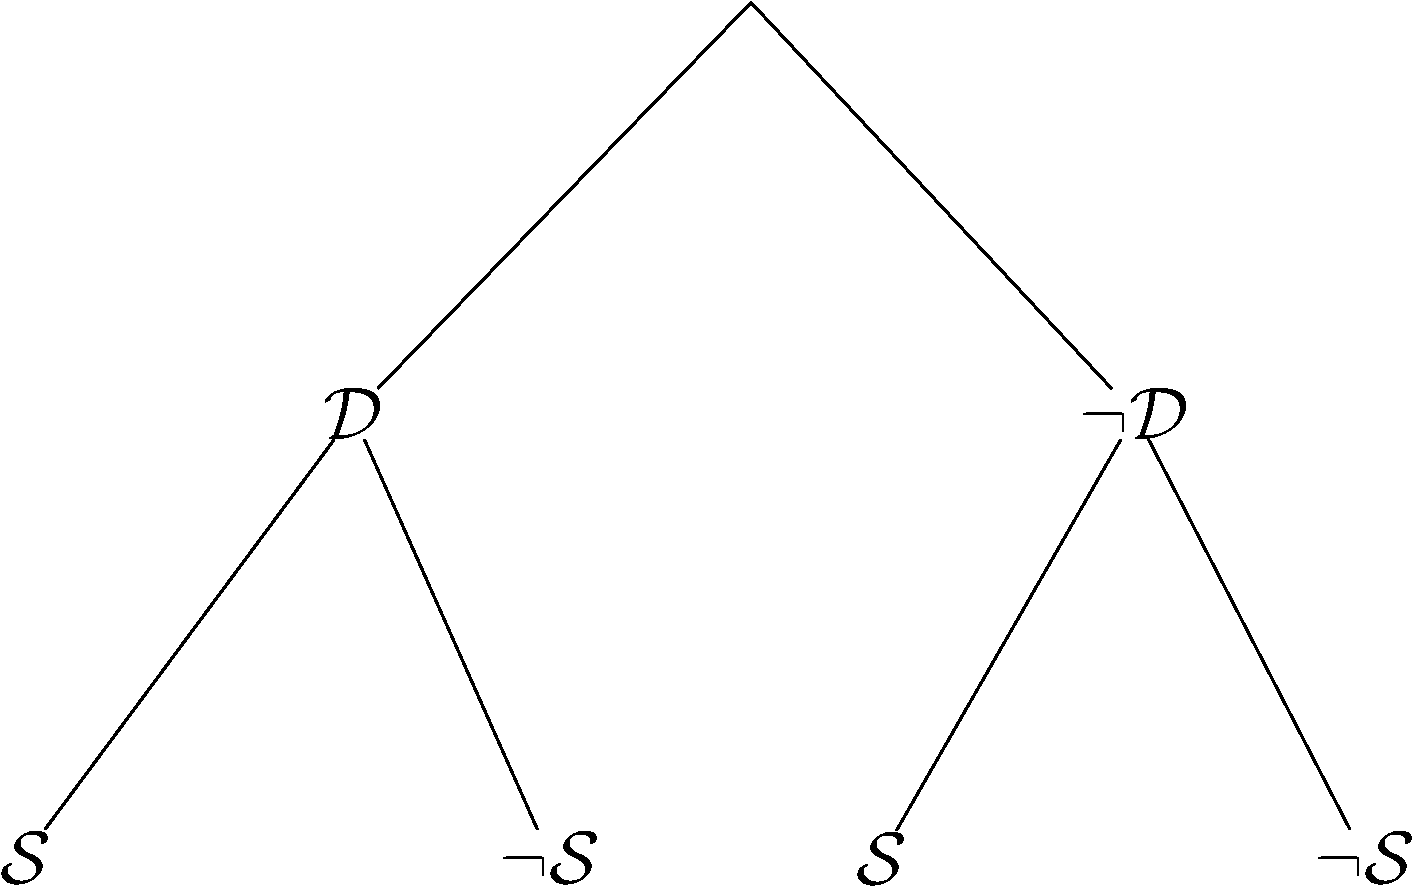
\includegraphics[width=\linewidth]{figures/treenoprobs}
\caption{A tree diagram of the events $\mathcal{D}$ (has a disease) and $\mathcal{S}$ (has a symptom).\label{fig:treenoprobs}}
\end{marginfigure}
Another way to think about marginalization is to draw a tree where you have the event, which you are marginalizing out ($\mathcal{D}$ in the previous exercise) at the first level of the tree and the variable you want to know the probability of ($\mathcal{S}$ in the previous exercise) at the next junction in the tree (see Figure~\ref{fig:treenoprobs}).


Further, we annotate the arrows with the conditional probability of the event conditioned on the things further up in the tree (note that for $\mathcal{D}$ there is nothing further up the tree, so we just write $p(\mathcal{D})$ or $p(\neg \mathcal{D})$).

\begin{center}
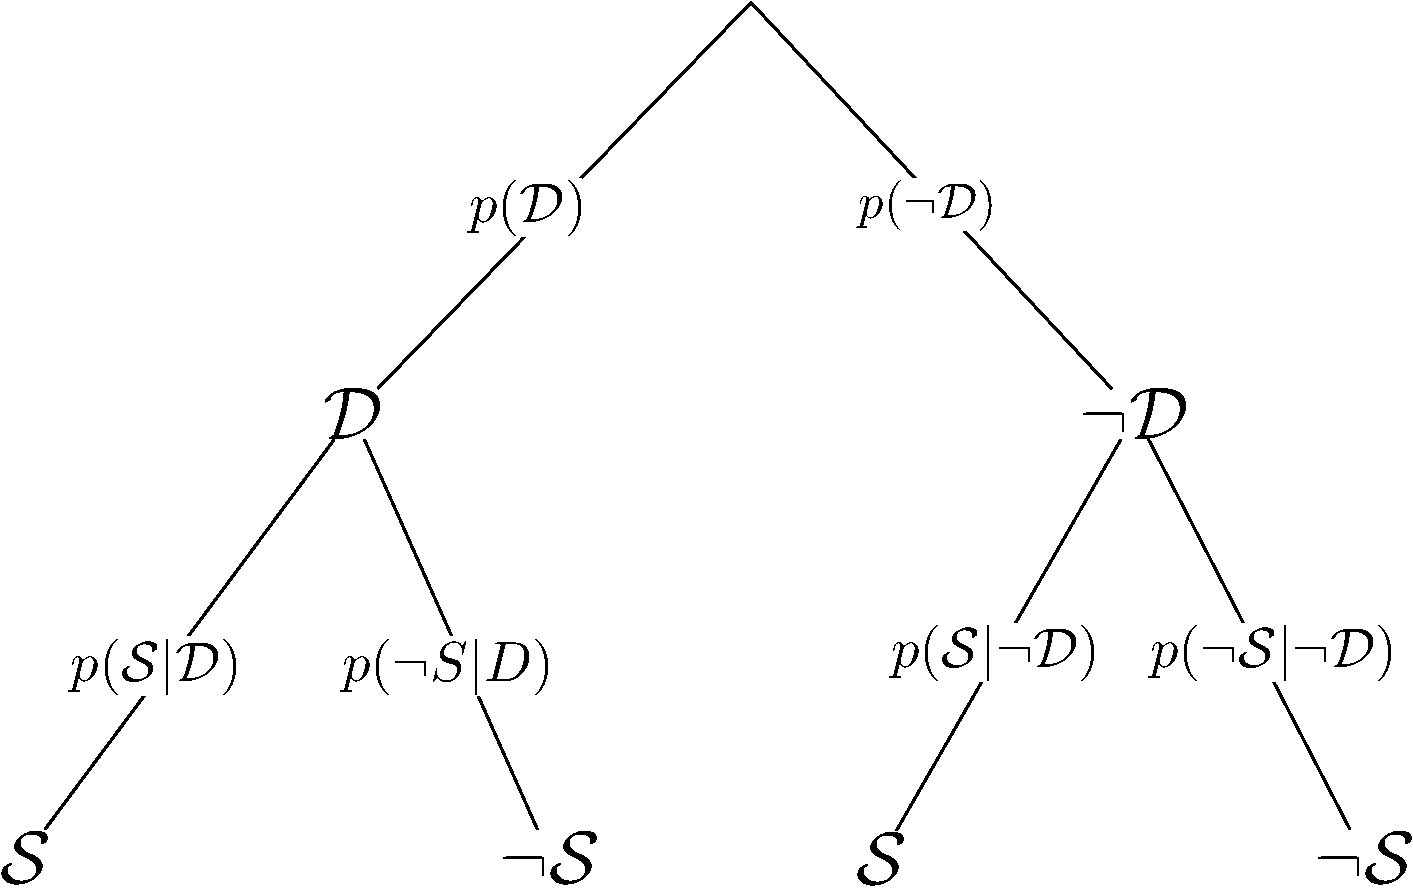
\includegraphics[width=0.6\linewidth]{figures/treeprobs}
\end{center}

If you want to find a joint probability (e.g., $p(\mathcal{D}, \neg \mathcal{S})$), follow the corresponding path, multiplying probabilities as you go.  For example, from examining the graph above we get
\begin{align}
p(\mathcal{D}, \neg \mathcal{S}) &= p(\mathcal{D}) p(\neg \mathcal{S}|\mathcal{D}) \enspace .
\end{align}

A marginal probability for an event (e.g., $p(\mathcal{S})$) can be found by summing over all paths that arrive at the event.  For example, from examining the graph above we see that there are two paths to $\mathcal{S}$, which allows us to compute $p(\mathcal{S})$ as
\begin{align}
p(\mathcal{S}) &= p(\mathcal{D}) p(\mathcal{S}|\mathcal{D}) + p(\neg \mathcal{D}) p(\mathcal{S}|\neg \mathcal{D})  \enspace .
\end{align}


\begin{exercise}[(20 minutes)]
Do problem 2 from \href{http://wwwf.imperial.ac.uk/~atw/Bayes.pdf}{this assignment}.  They use $\mathcal{E}'$ to refer to the event $\neg \mathcal{E}$.
\begin{boxedsolution}
Solution is embedded in the link.
\end{boxedsolution}
\end{exercise}

\section{Random Variables}

We've talked about the concept of an event that captures whether something happens as a result of some random process.  It turns out that it is very useful in machine learning and probabilistic modeling to talk about a variable that captures some quantity that is a result of some random process.  We call this entity a \emph{random variable}.

\begin{externalresources}[(20 minutes)]
Watch the following two videos from Khan Academy on Random Variables.
\bi
\item \href{https://www.khanacademy.org/math/statistics-probability/random-variables-stats-library/random-variables-discrete/v/random-variables}{Khan Academy Video on Random Variables}.
\item \href{https://www.khanacademy.org/math/statistics-probability/random-variables-stats-library/random-variables-discrete/v/discrete-and-continuous-random-variables}{Discrete and Continuous Random Variables} (note: for now we are interested in discrete random variables).
\ei
\end{externalresources}

Now that you have a sense of what a random variable is, we'll introduce the notion of probability mass function (or PMF).  A PMF is a function that assigns a probability to a discrete random variable taking on a particular value.  We'll use capital, unbolded letters to refer to random variables (e.g., the random variable $X$) and $p(X = k)$ to refer to the probability that $X$ takes on value $k$).

For example, if we were flipping a fair coin 3 times, we might define a random variable $X$ as follows.

\begin{align}
X&= \mbox{the number of coins that come up heads in 3 flips}
\end{align}

The probability mass function (PMF) is then defined over all possible values that $X$ could possibly take on.  If you don't know how we arrived at these values, that is fine.  These are results that can be derived using basic \href{https://en.wikipedia.org/wiki/Combinatorics}{combinatorics} (go take Sarah Spence Adams' class and learn how to do this).

\begin{align}
p(X=0) &= p(\mbox{0 heads come up}) = \frac{1}{8} \nonumber \\
p(X=1) &= p(\mbox{1 heads come up}) = \frac{3}{8} \nonumber \\
p(X=2) &= p(\mbox{2 heads come up}) = \frac{3}{8} \nonumber \\
p(X=3) &= p(\mbox{3 heads come up}) = \frac{1}{8} \nonumber 
\end{align}

We don't have an exercise for you to do here, but it is important for you to understand what a PMF is when digging into the companion notebook.

\section{Basic Bayes in Python}
\begin{externalresources}[(30 minutes)]
Go through the \href{https://colab.research.google.com/github/mlfa19/assignments/blob/master/Module\%202/01/Assignment_1_Companion_Notebook.ipynb}{assignment 1 companion notebook}.
\end{externalresources}

\companionnotebook{Assignment_1_Companion_Notebook}



\end{document}
